\graphicspath{{./SecondTask/}} % path to graphics

\section*{\LARGE Цель практической работы}
\addcontentsline{toc}{section}{Цель практической работы}

\textbf{Цель работы:} изучить основные элементы и правила построения диаграммы
вариантов использования.

\textbf{Задачи:}\par
\begin{itemize}
	\item изучить предметную область по заданным вариантам;
	\item определить на концептуальном уровне состав элементов системы в
		виде классов анализа;
	\item определить статическую структуру системы на логическом уровне,
		используя различные типы отношений;
	\item построить диаграмму, найти альтернативные варианты реализации
		системы (подсистемы).
\end{itemize}

\newpage

\section*{\LARGE Выполнение практической работы}
\addcontentsline{toc}{section}{Выполнение практической работы}
\section{Построение диаграммы классов анализа}
В вариантах использования работы банкомата (рис. \ref{fig:use_case})
, клиент банка может, например:
\begin{itemize}
	\item подписка на товар;
	\item покупка товара;
\end{itemize}
\begin{figure}[h!tp]
	\centering
	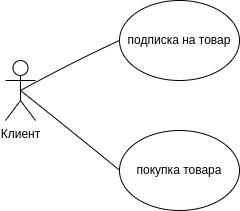
\includegraphics[width=0.6\textwidth]{uml_use_case.png}
	\caption{Варианты использования для работы аптеки}
	\label{fig:use_case}
\end{figure}

\section{Вариант использования "<покупка товара">}
В первую очередь выберем наиболее важный из перечисленных
вариантов использования, включим его в модель анализа, определим для него
классы анализа (классификаторы) и определим отношений между ними.
В качестве наиболее важного варианта использования выберем вариант
"<покупка товара">, в котором участвуют четыре класса (рис. \ref{fig:buy}):
\begin{itemize}
	\item поисковая строка --- граничный класс;
	\item доставка --- граничный класс;
	\item оплата --- управляющий класс;
	\item склад --- класс сущности.
\end{itemize}
\begin{figure}[h!tp]
	\centering
	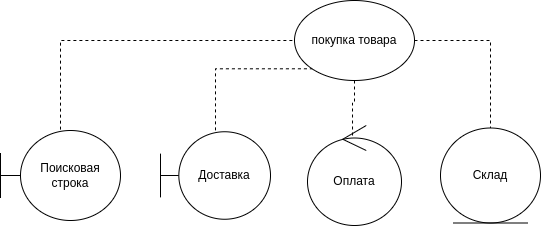
\includegraphics[width=0.8\textwidth]{uml_buy}
	\caption{Состав классов варианта использования "<покупка товара">}
	\label{fig:buy}
\end{figure}

Установим отношения между классами варианта использования
"<покупка товара"> (рис. \ref{fig:buy:impl}).
\begin{figure}[h!tp]
	\centering
	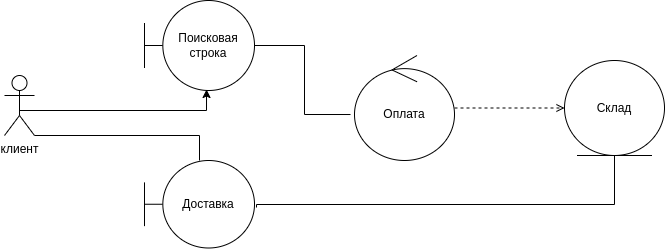
\includegraphics[width=0.8\textwidth]{uml_buy_impl}
	\caption{Реализации варианта использования "<покупка товара">}
	\label{fig:buy:impl}
\end{figure}

\section{Вариант использования "<подписка на товар">}
Повторим первые два шага для варианта использования
«Перечислить деньги на другой счет» (рис. \ref{fig:subscription}),
выделим классы (возможно новые классы анализа) и установим отношения
между ними. В варианте использования "<подписка на товар"> участвуют классы:
\begin{itemize}
	\item личный кабинет пользователя --- граничный класс;
	\item доставка --- граничный класс;
	\item БД пользователей --- класс сущности;
	\item склад --- класс сущности;
	\item оплата --- управляющий класс.
\end{itemize}
\begin{figure}[h!tp]
	\centering
	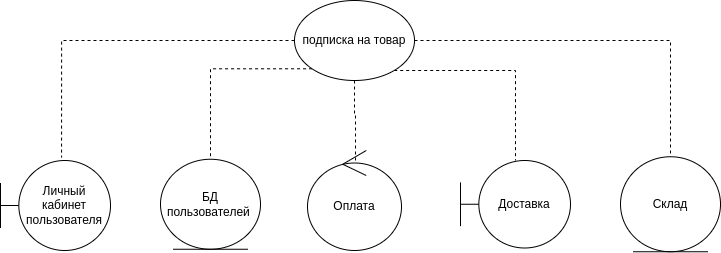
\includegraphics[width=0.8\textwidth]{uml_subscription}
	\caption{Состав классов варианта использования "<подписка на товар">}
	\label{fig:subscription}
\end{figure}

Установим отношения между классами варианта использования "<подписка на товар">
точно также, как и в шаге 2 (рис. \ref{fig:subscription:impl}).
\begin{figure}[h!tp]
	\centering
	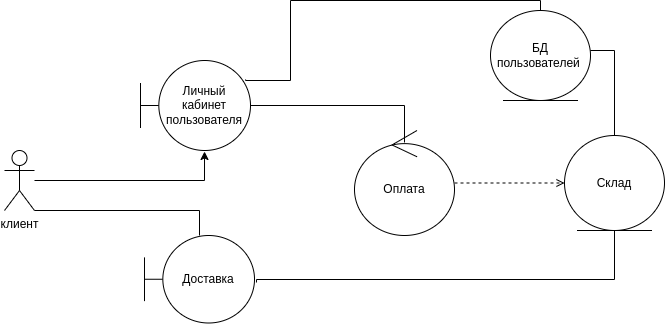
\includegraphics[width=0.8\textwidth]{uml_subscr_impl}
	\caption{Реализации варианта использования "<подписка на товар">}
	\label{fig:subscription:impl}
\end{figure}

\section{Итоговая диаграмма}
Создадим итоговую диаграмму классов анализа (рис. \ref{fig:complite}).
На рисунке видим классы, участвующие в нескольких реализациях варианта
использования модели анализа.
\begin{figure}[h!tp]
	\centering
	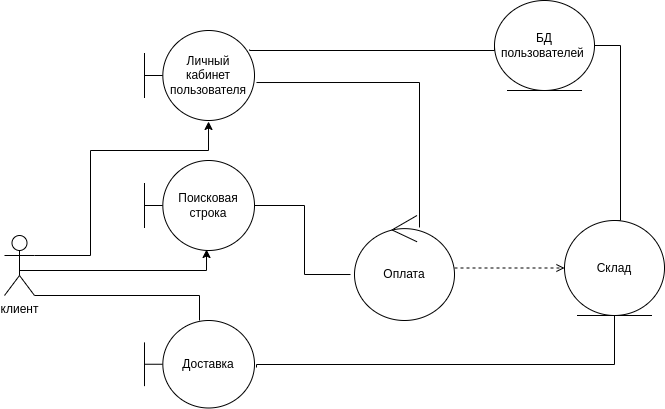
\includegraphics[width=0.8\textwidth]{uml_complite}
	\caption{Реализации варианта использования "<подписка на товар">}
	\label{fig:complite}
\end{figure}

\newpage

\section*{\LARGE Вывод}
\addcontentsline{toc}{section}{Вывод}
В результате практическои работы была создана диаграмма классов анализа,
идентифицированна обязанности участвующих классов анализа и определили
отношения между ними. Доставка, оплата и склад участвуют и
исполняют роли во всех трех реализациях вариантов использования. Видно,
что некоторые из классов могут оказаться новыми или изменившимися ролями
уже обнаруженных классов анализа, в то время как другие роли потребуют
новых классов анализа.\par
При проектировании классов анализа по различным стереотипам требуются
различные навыки и технологии. Так, например, проектирование классов
сущностей обычно требует использования технологий баз данных, в то время
как проектирование граничных классов — использования технологий
пользовательского интерфейса. Однако классы анализа с их ответственностями,
атрибутами и связями используются в качестве (логических) исходных данных
для создания соответствующих операций, атрибутов и отношений классов
проекта.
